% !TEX root = SegwayDoku.tex
\renewcommand{\autoren}{Stephan Morongowski}
\newpage
\section{Definition eines roboterfesten Koordinatensystems}

\begin{figure}[h]  % [h] bedeutet, dass das Bild genau an dieser Stelle im Text erscheint
\centering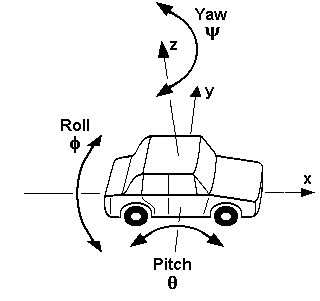
\includegraphics[width=0.6\textwidth]{images/FahrzeugKSys_mod.png}
\caption[Roboterkoordinatensystem]{Roboterkoordinatensystem \newline (Quelle: \cite{roboterKS_Bild})}
\label{robotKSys}
\end{figure}

Zur einheitlichen Bezeichnung wurde das roboterfeste Koordinatensystem (im Folgenden mit KS bezeichnet) wie in Abbildung \ref{robotKSys} zu sehen, ähnlich ISO 88551 festgelegt. Entgegen der häufig anzutreffenden Bezeichnungen der Winkel um die jeweiligen Koordinatenachsen werden im Folgenden die Winkel um
\begin{itemize}
    \item die x-Achse mit \(\alpha\)
    \item die y-Achse mit \(\beta\)
    \item die z-Achse mit \(\gamma\)
\end{itemize}
bezeichnet. \\
Der Ursprung des KS liegt auf der Radachse mittig zwischen den beiden Rädern.\\
Das KS ist ein rechtshändiges KS.\\\\
Die Verdrehung der jeweiligen Räder wird mit \(\varphi_l\) bzw. \(\varphi_r\) bezeichnet. Dabei bezeichnet \(l\) das in positive x-Richtung blickend links liegende Rad und \(r\) das in positive x-Richtung blickend rechts liegende Rad.

\newpage
